\section{Implications for the optimization of resource consumption and responsiveness trade-offs in \ac{WCA}}\label{sec:implications:optimization}

As with any application intended for mass deployment on multi-tenant systems such as the edge, \ac{WCA} applications will have to be configured and designed to minimize resource consumption at runtime.
At the same time, imposing too stringent requirements on resource consumption can adversely affect application responsiveness, which in turn has the potential to drastically reduce quality of experience for users.
Optimizing the deployment of these applications thus intrinsically involves achieving a balance between the reduction of resource consumption while maintaining an acceptable level of system responsiveness.

In the following section we will study the optimization of resource consumption-responsiveness trade-offs in two dimensions of \ac{WCA}, number of samples captured per step and energy consumption per step.

% \todo[inline]{Finish}

\subsection{Optimization framework}\label{ssec:optframework}

Our optimization approach focuses on the individual steps which comprise a complete \ac{WCA} task.
Thus, we begin by assuming a given execution time distribution \( \mathcal{T} \), and take the modeling and partial solution approach from recents works on energy efficient sampling in edge-based feedback systems.
In \textcite{Moothedath2021EnergyOptimal,Moothedath2022EnergyEfficient}, the authors model the energy in terms of the expected number of samples $\mathbb{E}[\mathcal{S}]$ and the expected wait time $\mathbb{E}[\mathcal{W}]$ experienced by the user.
The authors then find the optimum periodic sampling interval that minimizes this energy, or equivalently the non-constant parts of this energy termed as \textit{Energy Penalty}.

% In this optimization, the constant parts are excluded as it does not affect the process.
With a value much smaller than the execution time of the event, the \ac{RTT} of the final sample is included in this constant part, which is why $\mathcal{W}$ is computed without it.
Next, in \textcite{Moothedath2022Aperiodic}, the author retains the model, removes the constraint of periodicity, and finds the optimum aperiodic sampling instants $\{t_n,\,n=1,2,\dots\}$ that minimize the same energy penalty.

In this work, we use the modeling from~\cite{Moothedath2022Aperiodic} to find the optimum \emph{aperiodic} sampling interval.
However, instead of using their two-step approach to find the solution which includes a recursive solution followed by a bisection algorithm, we develop a novel, approximate, but easier solution to finding the set of the optimum aperiodic sampling intervals.
Furthermore, instead of directly optimizing for energy, we start by noting that an objective metric of a variety of optimization problems that are related to sampling, RTT, responsiveness or wait time present themselves 
% in a format similar to that of the energy, 
as a linear combination between $\mathbb{E}[\mathcal{S}]$ and $\mathbb{E}[\mathcal{W}]$ plus terms independent of the number of samples or wait time.
Let $\mathcal{E}$ correspond to such an objective metric.
Thus,
\begin{alignat}{1}
    \Rightarrow\mathcal{E}&=\alpha\mathbb{E}[\mathcal{S}]+\beta\mathbb{E}[\mathcal{W}]+C,\;\label{eq:epsilon_terminal}
\end{alignat}

Above, $\alpha, \beta$ and $C$ are constants which are responsible for modifying the objective function from one metric to another.
For instance, in the modeling used by \textcite{Moothedath2021EnergyOptimal,Moothedath2022EnergyEfficient,Moothedath2022Aperiodic}, the chosen characterization results in a metric which is equal to the energy penalty.
The outline of our solution that minimizes \cref{eq:epsilon_terminal} is provided below with the complete mathematical derivation in \cref{appx1}.

\bigskip

We first define an instantaneous sampling rate function $r(t)$ which is related to $\{t_n\}$ such that,
\begin{alignat}{1}
{\int_{t_{n-1}}^{t_n}}r(t)\dif t=1,\;\forall n\geq1\label{rt}
\end{alignat}
For instance, for periodic sampling, the rate function is a constant equal to the sampling frequency. 
% Using this rate function, we rewrite the expected number of samples as
% \begin{alignat}{1}
% \mathbb{E}[\mathcal{S}]&=\int_{t=0}^{\infty}\bigg(\!\int_{x=0}^{t}\!\!\!\!r(x)\,\mathrm{d}x\bigg)f_{\mathcal{T}}(t)\,\mathrm{d}t,\nonumber
% \end{alignat}
% and the approximate the expected wait time as
% \begin{alignat}{1}
% \mathbb{E}[\mathcal{W}]&=\int_{0}^{\infty}\dfrac{1}{2r(t)}f_\mathcal{T}(t)\,\mathrm{d}t.\nonumber
% \end{alignat}
Next, rewriting \cref{eq:epsilon_terminal} in terms of $r(t)$ and minimizing it gives as an optimum rate function $r^*(t)$ as
\begin{alignat}{1}
r^*(t)&=\sqrt{\dfrac{\beta f_\mathcal{T}(t)}{2\alpha\bar{F}_\mathcal{T}(t)}}\nonumber\\
\intertext{in turn resulting in, for a $\mathcal{T}$ distributed according to a Rayleigh distribution with parameter $\sigma$,}
r^*(t)&=\sqrt{\dfrac{\beta t}{2\alpha\sigma^2}}\nonumber\\
% \Rightarrow &\int_{t_n}^{t_{n+1}}\!\!\!\sqrt{\dfrac{\beta t}{2\alpha\sigma^2}}\,\mathrm{d}t=1,\;\forall n\geq1\nonumber\tag{from \eqref{rt}}\\
% \Rightarrow &\;t_{n+1}^{\frac{3}{2}}-t_{n}^{\frac{3}{2}}=3\sigma\!\sqrt{\tfrac{\alpha}{2\beta}}\nonumber\\
\Rightarrow t_n&=\Big(3\sigma\!\sqrt{\tfrac{\alpha}{2\beta}}\Big)^{\frac{2}{3}}n^{\frac{2}{3}}\label{tn_approx_rayleigh}
\end{alignat}


\subsection{Optimizing for mean number of samples per step}\label{ssec:optimization:samples}

We first look at the application of \cref{eq:epsilon_terminal} for the optimization of number of captured samples per step.
We start with this metric as its implications for resource consumption and responsiveness are straightforward to understand.
On the one hand, higher sampling rates directly lead to perceived increased system responsiveness, as smaller sampling intervals translate into smaller maximum wait times.
On the other, the relationship between number of samples captured and sent and network congestion is exponential, and too high sampling rates quickly lead to bottlenecks on the network, particularly in multi-tenant environments.
Additionally, the energy cost of capturing a sample on a \ac{WCA} client device is often much higher than remaining in an idle state, and thus excessive sampling leads to drastically increased energy consumption.
Optimizing the number of samples captured per step can thus be a straightforward way of reducing resource consumption and contention in \ac{WCA} applications.

However, an unconstrained optimization of the number of samples is trivial and meaningless as the solution points to a single sample at $t\!\rightarrow\!\infty$, which also takes the wait time to infinity.
We look at the constrained optimization of the expected number of samples with an upper bound $w_0$ for the expected wait.
That is, $\mathbb{E}[\mathcal{W}]\!\leq\!w_0$. We show in \cref{appx1} that the appropriate $\alpha$ and $\beta$ for this problem satisfy the condition
\begin{alignat}{1}\label{eq:optimization:sampling}
\frac{\alpha}{\beta}=\frac{2\sqrt{2}\,w_0^2}{(\mathlarger{\Gamma}(\tfrac{3}{4}))^2\,\sigma}\approx1.9\frac{w_0^2}{\sigma}
\end{alignat}
where, $\mathlarger{\Gamma}(x)$ is the Gamma function.

\medskip

We introduce here a reference scheme to which we will compare our approach.
In~\cite{Wang2019Towards}, \citeauthor{Wang2019Towards} introduce an adaptive sampling scheme for \ac{WCA} intended to reduce the number of samples processed per step while still meeting application responsiveness bounds.
At every sampling instant \( t \), the scheme adapts the sampling rate \( R(t) \) of the system according to the estimated likelihood of the user having finished the step,
following the formula 

\begin{equation}
    R(t) = R_\text{min} + \varphi\left( R_\text{max} - R_\text{min} \right) * CDF(t)
\end{equation}

\( R_\text{max} \) and \( R_\text{min} \) correspond to the maximum and minimum sampling rates of the system, respectively.
\( R_\text{max} \) can directly be assumed to correspond to \( 1 / \text{\ac{RTT}}_\mu \), where \( \text{\ac{RTT}}_\mu \) corresponds to the mean \ac{RTT} of the system.
\( R_\text{min} \) needs to either be calculated according to the latency bounds of the system or specified manually.
\( \varphi \) corresponds to a scaling factor and \( t \) to the time of the current sampling instant with respect to the start of the step.
Finally, \( CDF \) corresponds to the \ac{CDF} of a distribution describing the execution times for the current step; \citeauthor{Wang2019Towards} used a single static Gaussian distribution for all steps in their work.

\medskip

In the following, we will show the effects of our optimization approach combined with our timing models compared to \textcite{Wang2019Towards}'s state-of-the-art approach.
For this we implement these sampling schemes in Python and run a number of simulations with them.
The first scheme uses our approach and \cref{eq:epsilon_terminal,eq:optimization:sampling} to determine the optimum sampling instants and the values for \( \alpha \) and \( \beta \) at each step.
It includes an embedded timing model (without any distribution fitting) to provide updated estimates of the mean execution time \( \mu \) and \( \sigma \) at every step as well, allowing it to adapt to the state of the system.
We will refer to this scheme as the \emph{sample-count-optimized aperiodic} sampling scheme.

We implement \citeauthor{Wang2019Towards}'s original design using a Gaussian distribution fitted to all the execution times collected for~\cite{olguinmunoz:impact2021} for \ac{CDF} calculation.
This scheme does not include an embedded timing model, and uses the same \ac{CDF} for every step.

Finally, we also implement two reference sampling schemes representing best- and worst-case extremes.
The first of these corresponds to the offline optimum which uses an embedded \emph{oracle} to perfectly predict the execution time of each step.
Such an ideal scheme is thus able to always sample exactly once per step, with a constant wait time of zero.
The second reference scheme corresponds to one which \emph{greedily} samples as much as possible.
This represents a completely unoptimized design with no considerations for resource-consumption trade-offs; it simply attempts to maximize the number of captured samples per step.
This is an interesting approach to include given that it corresponds to the default sampling strategy used in most existing \ac{WCA} prototypes.

\begin{table}
    \centering
    \caption{Experimental parameters}\label{tab:params}
    \begin{tabular}{lrl}
        \toprule
        Parameter & Value & Clarification \\
        \midrule
        \# of steps & \num{100} & \\
        Repetitions & \num{100} & \\
        \acp{RTT} & \( \left\{ 0.3, 0.6,\ldots,4.2 \right\} \) & \\
        \( \tau_\text{p} \) & \SI{250}{\milli\second} & Processing delay \\
        \( \tau_\text{c} \) & \( \text{\ac{RTT}} - \tau_\text{p} \) & Communication delay \\
        \( w_0 \) & \SI{1.0}{\second} & \\
        \( R_\text{min} \) & \SI{0.5}{\hertz} & Derived as \( R_\text{min} = {(2 w_0)}^{-1} \) \\
        \( \varphi \) & \num{1.5} & Scaling factor, \textcite{Wang2019Towards}\\
        \( P_0 \) & \SI{15}{\milli\watt} & Idle power \\
        \( P_\text{c} \) & \SI{45}{\milli\watt} & Communication power \\
        \( \alpha_\text{samples} \) & \( 1.9 \sigma^{-1} \) & For sample-count optimization. \\
        \( \beta_\text{samples} \) & \num{1.0} & For sample-count optimization. \\
        \( \alpha_\text{energy} \) & \( \tau_\text{c}(P_\text{c} - P_0) \) & For energy optimization. \\
        \( \beta_\text{energy} \) & \( P_0 \) & For energy optimization. \\
        \bottomrule
    \end{tabular}
\end{table}

We proceed to set up an experiment where these sampling approaches are deployed on identical, simulated, tasks with varying constant \acp{RTT}.
Experimental parameters are summarized in \cref{tab:params}.
We set the \( w_0 \) and \( \beta \) factors of our sample-count-optimized scheme to \SI{1.0}{\second} and \num{1.0}, respectively, for mathematical simplicity, and derive \( \alpha = 1.9 \sigma^{-1} \).
Next, we derive \( R_\text{min} \) for \textcite{Wang2019Towards}'s scheme from \( w_0 \).
As discussed in \cref{sec:background}, we assume that wait times are uniformly distributed between \SI{0}{\second} and sampling interval of each step.
A maximum expected wait time \( w_0 = 1.0\,\si{\second} \) thus translates into a maximum expected sampling interval of \SI{2.0}{\second}, yielding a minimum sampling rate \( R_\text{min} = {2.0\,\si{\second}}^{-1} = 0.5\,\si{\hertz} \).


The execution times for each step are generated by a timing model without any distribution fitting on the data.
For each combination of sampling scheme configuration, \ac{RTT}, and execution time model neuroticism (low or high), we run \num{100} repetitions of the task for good statistical significance.
Note that the embedded timing model in our sampling-count-optimized aperiodic sampling scheme is always parameterized with a neuroticism matching the neuroticism of the external execution time model.

\begin{figure*}
    \centering
    \begin{subfigure}[t]{\textwidth}
        \centering
        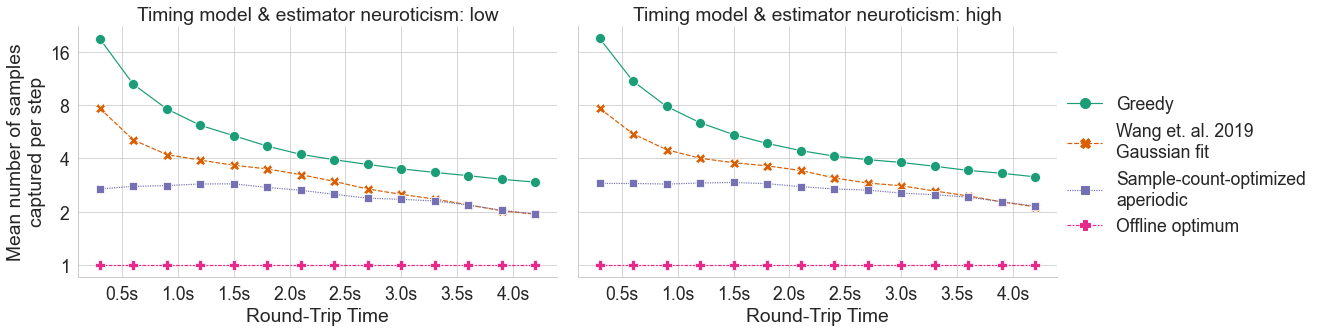
\includegraphics[width=\textwidth]{figs/new_model/sampling_optimization.png}
        \caption{%
            Round-trip time versus mean number of captured samples per step, averaged over all \num{100} repetitions of the experiment.
            Note the logarithmic scale on the vertical axis.
            Error bars indicate \SI{95}{\percent} \acp{CI}.
        }
    \end{subfigure}\\
    \medskip
    \begin{subfigure}[t]{\textwidth}
        \centering
        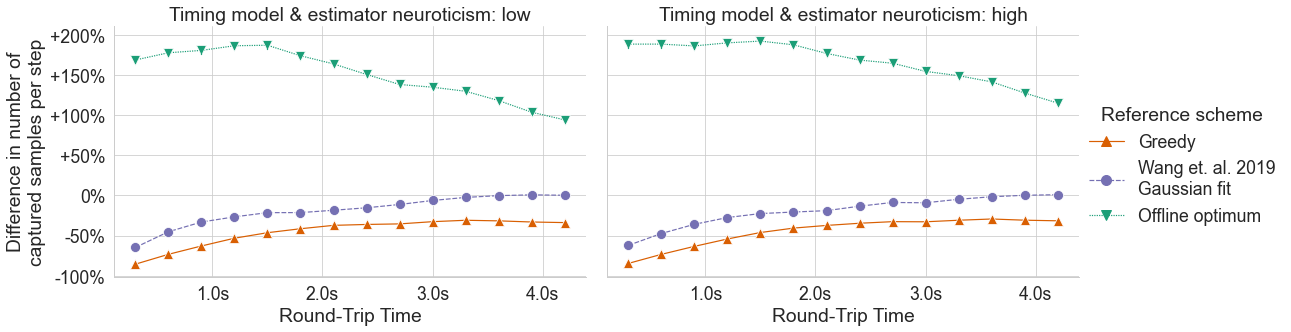
\includegraphics[width=\textwidth]{figs/new_model/sampling_optimization_diff.png}
        \caption{%
            Percentage difference in mean number of captured samples per step with respect to the greedy sampling scheme.
            Error bars indicate \SI{95}{\percent} \acp{CI}, calculated using a two-sided t-test.
        }
    \end{subfigure}
    \caption{%
        Summary of results for experiment comparing the sample-count-optimized aperiodic sampling scheme to the reference schemes and \textcite{Wang2019Towards}'s \ac{CDF}-based approach.
    }\label{fig:optimization:samples}
\end{figure*}

The results of this investigation are presented in \cref{fig:optimization:samples}.
\todo[inline]{Discuss results.}

\subsection{Optimizing for energy consumption}\label{ssec:optimization:energy}

Next we will explore the implications of combining our timing models with \cref{eq:epsilon_terminal} when directly optimizing for energy consumption in \ac{WCA}.
Although, as mentioned above, minimizing the number of samples captured during a step can \emph{potentially} translate into a reduction in the energy consumption, this is not a given.
Energy consumption depends on multiple other factors other than number of samples captured, such as idle versus communication power and delays, and thus cannot be optimized by simply minimizing the number of samples taken.

In the following we thus take the general solution, \cref{eq:epsilon_terminal}, and find the appropriate \( \alpha \) and \( \beta \) to minimize the energy consumed per step, i.e.\ \( \mathcal{E}=E \).
We directly take the modeling from~\cite{Moothedath2022Aperiodic} with a necessary modification in the assumption of one-way communication in all but the final sample.
With feedback given even to the discarded samples in our model, we have, 
\begin{alignat}{2}
    \mathrm{E}=&\;2\mathcal{S}\tau_cP_c+(\mathcal{T}+\mathcal{W}+\tau_\mathrm{p}+2\tau_\mathrm{c}-2\mathcal{S}\tau_c)P_0\nonumber\\
    % &=s\tau_c(P_c-P_0^{(t)})+wP_0^{(t)}+(\tau+\tau_c+\tau_p) P_0^{(t)}+\tau_cP_c\\
    =&\;2\tau_{\text{c}}(P_{\text{c}} -P_0)\mathcal{S}+\mathcal{W}P_0+(\mathcal{T}+\tau_{\text{p}} +2\tau_{\text{c}}) P_0\nonumber\\
&\Rightarrow \alpha=2\tau_{\text{c}}(P_{\text{c}} -P_0),\text{ and }\beta=P_0 \label{eq:optimization:energy}
\end{alignat}
\( \tau_\text{p} \) and \( \tau_\text{c} \) correspond to the processing and communication delay for each sample.
\( P_\text{c} \) and \( P_0 \) correspond to the communication and idle power, respectively, of the \ac{WCA} client device.

We proceed to repeat the experiment detailed in \cref{ssec:optimization:samples}, replacing the sample-count-optimized sampling scheme with a new implementation instead minimizing energy, using \cref{eq:optimization:energy} for the calculation of \( \alpha \) and \( \beta \).
Once again, we embed a timing model into the sampling scheme to provide updated estimates of the mean execution time \( \mu \) at each step.
We refer to this scheme as the \emph{energy-optimized aperiodic} sampling scheme.
For the power constants, we reuse the values estimated by the authors in \textcite{Moothedath2022EnergyEfficient}, \( P_\text{c} = 45\,\si{\milli\watt} \) and \( P_\text{0} = 15\,\si{\milli\watt} \).
On the other hand, for the timing variables we define a constant processing delay \( \tau_\text{p} = 250\,\si{\milli\second} \) across all configurations and repetitions of the experiments; given then a constant \ac{RTT} for the task, we set \( \tau_\text{c} = \text{\ac{RTT}} - \tau_\text{p} \).

\begin{figure*}
    \centering
    \begin{subfigure}[t]{\textwidth}
        \centering
        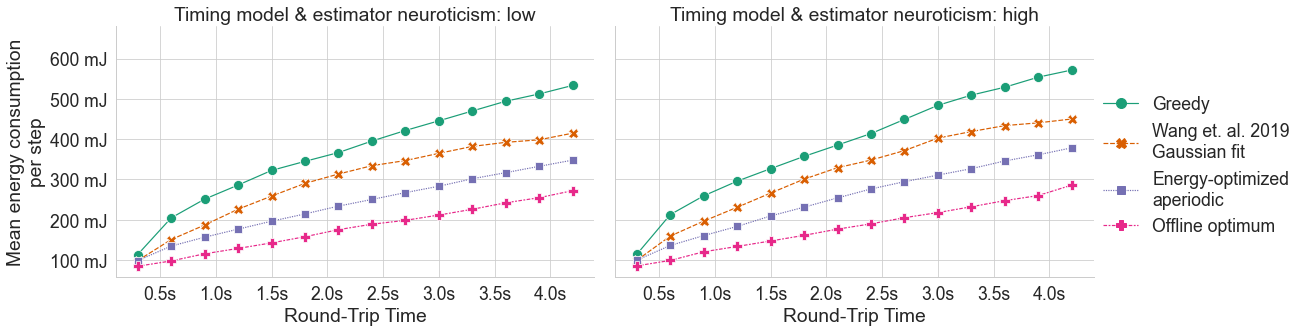
\includegraphics[width=\textwidth]{figs/new_model/energy_optimization.png}
        \caption{%
            Round-trip time versus mean per step energy consumption, averaged over all \num{100} repetitions of the experiment.
            Error bars indicate \SI{95}{\percent} \acp{CI}.
        }
    \end{subfigure}\\
    \medskip
    \begin{subfigure}[t]{\textwidth}
        \centering
        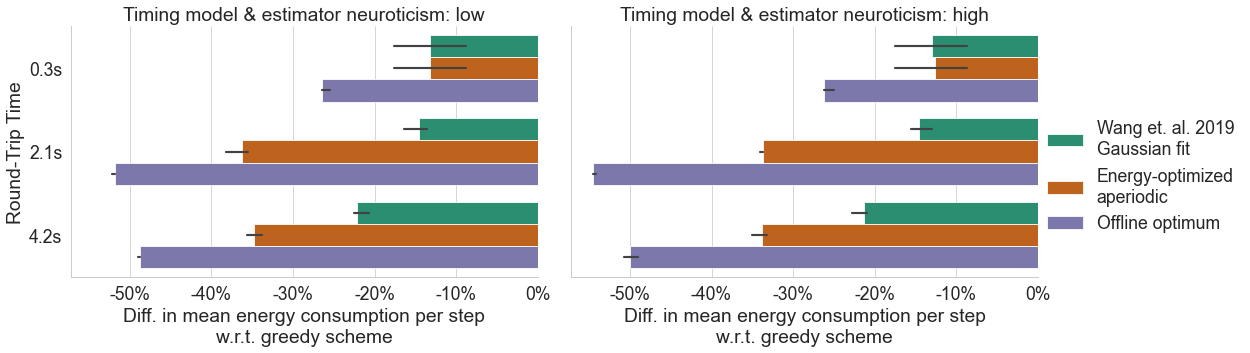
\includegraphics[width=\textwidth]{figs/new_model/energy_optimization_diff.png}
        \caption{%
            Percentage difference in mean per step energy consumption with respect to the greedy sampling scheme.
            Error bars indicate \SI{95}{\percent} \acp{CI}, calculated using a two-sided t-test.
        }
    \end{subfigure}
    \caption{%
        Summary of results for experiment comparing the energy-optimized aperiodic sampling scheme to the reference schemes and \textcite{Wang2019Towards}'s \ac{CDF}-based approach.
    }\label{fig:optimization:energy}
\end{figure*}

Again, we include the reference greedy and offline optimum schemes, as well as \textcite{Wang2019Towards}'s approach, and repeat the experiment \num{100} times for each combination of sampling scheme, neuroticism, and \ac{RTT}.
The results of these experiments are presented in \cref{fig:optimization:energy}.

\todo[inline]{Discussss}